\chapter{Harmonic Oscillations}

\textit{Each thing... comes round again in its cycle.}
Marcus Aurelius

\begin{marginfigure}%
  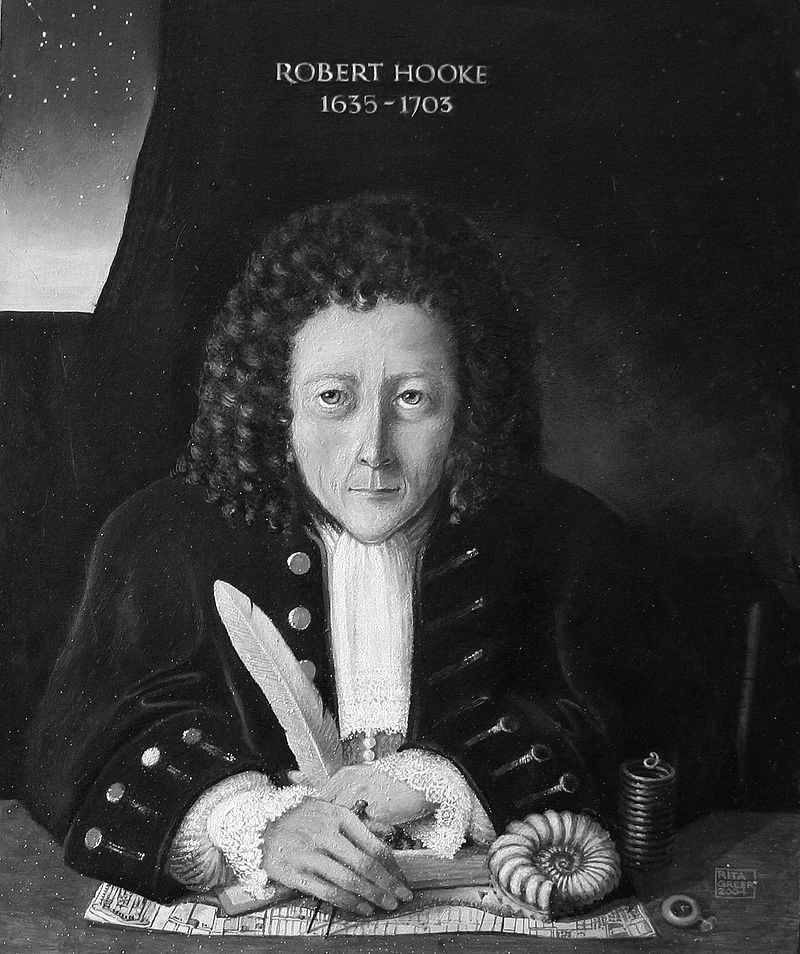
\includegraphics[width=\linewidth]{hooke.jpg}
  \caption{Portrait of Robert Hooke.}
  \label{fig:marginfig}
\end{marginfigure}
\marginnote{As no contemporary portrait of Robert Hooke seems to have survived from the seventeenth century, this one is a reconstruction from the descriptions by his colleagues Aubrey and Waller. It shows him with a spring, pocket watch, fossil and map of the City of London after the Great Fire of 1666. He helped to survey and plan the rebuilding. The sky on the left indicates his interest in astronomy.}


\section{Simple Harmonic Motion}
\subsection{Hooke's Law}

Hooke's law represents a linear restoring force to a point of equilibrium.  This is a model for the ideal spring.  The constant of proportionality, $k$, between the force and displacement is called the spring constant.  For other linear systems $k$ is used to represent the constant of proportionality and simply referred to as the $k$ constant.
$$F_{spring}=-kx$$
This physical system behaves according to a differential kinematic relationship.  Specifically the acceleration has a negative proportionality to the position.
$$F_{spring}=F_{net}=ma$$
$$m \lim_{\Delta \rightarrow 0} \frac{\Delta v}{\Delta t}=-kx$$
$$\lim_{\Delta \rightarrow 0} \frac{\Delta (\Delta x / \Delta t)}{\Delta t}=-\frac{k}{m}x$$
$$a=-\frac{k}{m}x$$

\begin{marginfigure}%

\begin{tikzpicture}[scale=0.6]
	\tikzstyle{spring}=[thick,decorate,decoration={zigzag,pre length=0.1cm,post length=0.1cm,segment length=6}]
	\draw[->,thick] (0,0) -- (0,1) node [anchor=south ,scale=1] {$F_{spring}$}; 
    	\fill[black] (0,0) circle (0.5mm);
	   
	\begin{scope}[shift={(-5,-1)}, scale=0.5]
		\draw[dashed, color=gray] (-3,2) -- (3,2) node [near start, anchor =south east] {\tiny equilibrium};
		\draw[spring] (0,1) -- (0,5);
		\draw[->,thick, color=gray] (2,2) -- (2,0) node [midway, anchor =west] {\small$\overrightarrow{x}$};
		\fill[color=gray!30, path fading=north] (-3,5) -- (3,5) -- (3,7) -- (-3,7) ;
		\draw[very thick] (-3,5) -- (3,5);  
		\draw[very thick] (-1,-1) -- (-1,1) -- (1,1) -- (1,-1) -- cycle;  	 
		\draw (0,0) node [anchor=center]{$m$};
   	 \end{scope}
   
   
   	  \begin{scope}[shift={(-2,0.2)}, scale=0.75, rotate=180] 
	  	\draw[ thick,-stealth] (0,-0.1) -- (0,0.8) node [near start,anchor=east]{\scriptsize $x$};  
	 	 \draw[thick](-0.1,0) -- (0.1,0);  
	  \end{scope}
	  
   \end{tikzpicture}
 
  \caption{Hookean system}
  \label{fig:marginfig}
\end{marginfigure}

   
\subsection{Equations of Motion}
$$x(t)=A\cos(\omega t)+B\sin(\omega t)$$
$$v(t)=-\omega A\sin(\omega t)+\omega B\cos(\omega t)$$
$$A=x_0\ \ \ \ \ \ B=\frac{v_0}{\omega}\ \ \ \ \ \ \omega=\sqrt{\frac{k}{m}}$$
\newpage
\subsection{Energy}
\begin{fullwidth}
The classical harmonic oscillator is a lovely system in terms of symmetry.  Kinetic and potential anergy have equal influence over the evolution of the system.  The inertial quantity $m$ weights the squared velocity to constitute the kinetic energy whereas the elastic quantity $k$ weights the squared distance to constitute the potential energy.

$$KE=\frac{mv^2}{2}\hspace{2cm}PE=\frac{kx^2}{2}$$
$$E=KE+PE$$
$$E=E_0=\frac{mv_0^2}{2}+\frac{kx_0^2}{2}=KE_{max}=PE_{max} \hspace{2cm} KE=E_0-PE=E_0 (\sin^2(2\omega t+\phi) ) $$
$$|v_{max}|=\sqrt{\frac{2E_0}{m}} \hspace{2cm} |x_{max}|=\sqrt{\frac{2E_0}{k}}$$


\section{Pendulum}

\footnotesize{

A pendulum is a weight suspended from a pivot so that it can swing freely.  When a pendulum is displaced sideways from its resting, equilibrium position, it is subject to a restoring force due to gravity that will accelerate it back toward the equilibrium position. When released, the restoring force combined with the pendulum's mass causes it to oscillate about the equilibrium position, swinging back and forth. The time for one complete cycle, a left swing and a right swing, is called the period. The period depends on the length of the pendulum, and also to a slight degree on the amplitude, the width of the pendulum's swing.}

\end{fullwidth}

\vspace{1cm}
\footnotesize{
Newton's second law for rotation of rigid bodies written below.  The net torque is equal to the product of the moment of inertia and the angular acceleration. }
$$\tau_{net}=I\alpha$$
\footnotesize{Substituting the torque and moment of inertia yields the following equation.}
$$mgl\sin{\theta}=ml^2\alpha$$
\footnotesize{The underlying differential relationship of the system is that the double time rate of change of the angle is the ratio of the restoring torque and the inertial moment.}
$$\lim_{\Delta \rightarrow 0} \frac{\Delta^2 \theta}{(\Delta t)^2}=-\frac{g}{l}\sin\theta$$


\begin{marginfigure}[-6cm]
$$\begin{tikzpicture}[scale=0.7]
   
	  \begin{scope}[shift={(-5,-1)}, scale=0.5]
	   \begin{scope}[shift={(1.5,5)}, scale=1, rotate=-20]
	    \draw[very thick] (0,0) -- (0,-5) node [midway, anchor=north east, scale=1] {$l \ \  $}; 
	     \draw[very thick] (0,-6) circle (1cm); 
	     \draw (0,-6) node [anchor=center]{$m$};
	   \end{scope}
	 
	   \draw[dashed] (1.5,5) -- (1.5,1.5) node [midway, anchor=north east] {\small$\theta$};; 
	  \fill[color=gray!30, path fading=north] (-3,5) -- (3,5) -- (3,7) -- (-3,7) ;
	  \draw[very thick] (-3,5) -- (3,5);  
	   
   	
   \end{scope}
   
   
   	  \begin{scope}[shift={(-2,0.2)}, scale=0.75, rotate=-20] 
	  \draw[ thick,-stealth] (0,-0.1) -- (0,0.8) node [near start,anchor=east]{\scriptsize $r$};  
	  \draw[thick](-0.1,0) -- (0.1,0);
	   \draw[thick](0.2,-0.4) -- (0.2,-0.6);
	    \draw[ thick,-stealth] (0.1,-0.5) -- (1,-0.5) node [near start,anchor=north]{\scriptsize $\theta$};  
	  \end{scope}
   \end{tikzpicture}$$


  \caption{Ideal pendelum}
  \label{fig:marginfig}
\end{marginfigure}

\begin{fullwidth}
\footnotesize{
From its examination in around 1602 by Galileo Galilei, the regular motion of pendulums was used for timekeeping, and was the world's most accurate timekeeping technology until the 1930s.  Pendulums are used to regulate pendulum clocks, and are used in scientific instruments such as accelerometers and seismometers. Historically they were used as gravimeters to measure the acceleration of gravity in geophysical surveys, and even as a standard of length. The word "pendulum" is new Latin, from the Latin pendulus, meaning 'hanging'.  The simple gravity pendulum is an idealized mathematical model of a pendulum.  This is a weight (or bob) on the end of a massless cord suspended from a pivot, without friction. When given an initial push, it will swing back and forth at a constant amplitude. Real pendulums are subject to friction and air drag, so the amplitude of their swings declines.
}
\end{fullwidth}

\vspace{1cm}

\subsection{Small Angle Approximation}
$$\sin \theta=\sum_{n=0}^{\infty} \frac{(-1)^n\theta^{2n+1}}{(2n+1)!}=\theta-\frac{\theta^3}{3!}+\frac{\theta^5}{5!}-\cdots$$
$$\lim_{\theta \rightarrow 0} \sin \theta \approx \theta$$

$$\lim_{\Delta \rightarrow 0} \frac{\Delta (\Delta \theta / \Delta t)}{\Delta t}\approx-\frac{g}{l}\theta$$

\marginnote[-4cm]{   
\subsection{Equations of Motion}
$$\Theta(t)=A\cos(\omega t)+B\sin(\omega t)$$
$$\Omega(t)=-\omega A\sin(\omega t)+\omega B\cos(\omega t)$$
$$A=\theta_0\ \ \ \ \ \ B=\frac{\dot{\theta}_0}{\omega}\ \ \ \ \ \ \omega=\sqrt{\frac{g}{l}}$$


\section{Magnitude and Phase}
$$A\cos(t)+B\sin(t)=R\cos(t+\phi)$$
$$R=\sqrt{A^2 + B^2} \hspace{2cm} \phi=\tan^{-1}\left(\frac{B}{A}\right)$$
}

\section{Damped Harmonic Oscillator}
\begin{marginfigure}%
  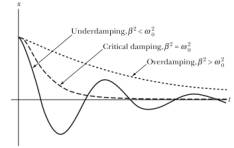
\includegraphics[width=\linewidth]{dampening.jpg}
  \caption{Solutions to the damped harmonic oscillation}
  \label{fig:marginfig}
\end{marginfigure}
\normalsize
The differential equation that represents the simple harmonic oscillator system is written below.
$$ma=-fx \hspace{2cm} ma+kx=0$$
This equations gives the following solution.
$$x(t)=A\cos(\omega t)+B\sin(\omega t) $$
The dampening occurs when a force is introduced that is proportional to the velocity.  This is the dampening force.
$$ma=-\beta v-kx$$
$$ma+\beta v+kx=0$$
This yields three types of solutions.
\subsection{Over-Damped}
In the case of over damping the dampening coefficient $\beta$ is above a certain threshold. 
$$\beta^2>4mk$$
This yields solutions of exponential decay as follows.
$$x(t)=Ae^{-\frac{\beta+\sqrt{\beta^2-4mk}}{2m}t}$$
\subsection{Critically-Damped}
In the case of critical damping the dampening coefficient $\beta$ equal to the threshold. 
$$\beta^2=4mk$$
This yields exponential decay as follows.
$$x(t)=Ae^{-\frac{\beta}{2m}t}$$
\subsection{Under-Damped}
In the case of under damping the dampening coefficient $\beta$ below the threshold. 
$$\beta^2<4mk$$
This yields solutions of decaying oscillation as follows.
$$x(t)=Ae^{-\frac{\beta}{2m}t}\cos(\omega t)+Be^{-\frac{\beta}{2m}t}\sin(\omega t)$$
$$A=x_0\ \ \ \ \ \ B=\frac{v_0+\nicefrac{\beta}{2m}}{\omega}\ \ \ \ \ \ \omega=\frac{\sqrt{\beta^2-4mk}}{2m}$$

\section{Driven Damped Harmonic Oscillator}
\begin{marginfigure}%
  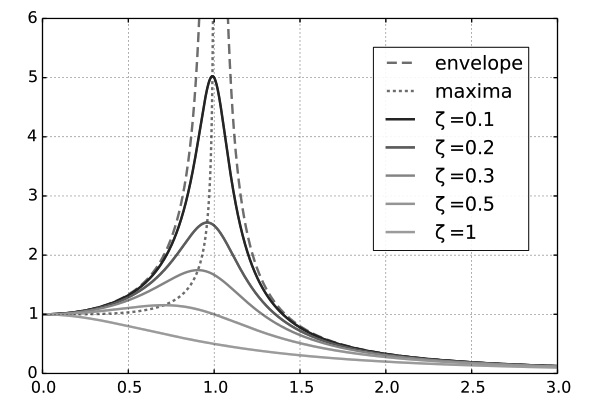
\includegraphics[width=\linewidth]{resonance.jpg}
  \caption{Amplitude at resonance}
  \label{fig:marginfig}
\end{marginfigure}
If a damped oscillator is driven by an external force, the solution to the motion equation has two parts, a transient part and a steady-state part, which must be used together to fit the physical boundary conditions of the problem.  The system will obey the following differential equation.  $F(t)$ is the driving force.
$$ma=-\beta v-kx+F(t)$$
$$ma+\beta v+kx=F(t)$$
The transient solutions go to zero after sufficient time and only the steady state solutions will remain.  The steady state solutions with follow the frequency of the driving force.  Resonance occurs if the frequency of the driving force matches the natural frequency of the system.  When this happens with insufficient dampening the driving force with continually add energy to the system until catastrophe occurs.

\section{Mechanical Resonance}
\begin{marginfigure}[100pt]
  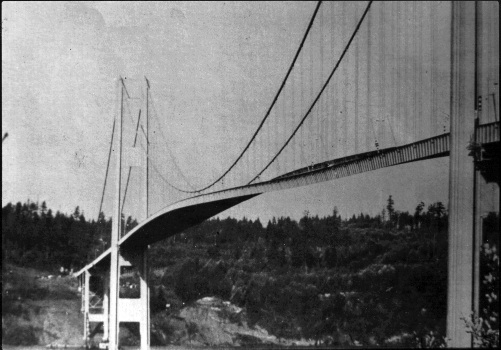
\includegraphics[width=\linewidth]{tacoma.jpg}
  \caption{Tacoma Narrows Bridge (1940)}
  \label{fig:marginfig}
\end{marginfigure}
\marginnote[20pt]{The original Tacoma Narrows Bridge roadway twisted and vibrated violently under 40-mile-per-hour winds on it's last day.  It collapsed on the morning of November 7, 1940.}
Mechanical resonance is the tendency of a mechanical system to respond at greater amplitude when the frequency of its oscillations matches the system's natural frequency of vibration (its resonance frequency or resonant frequency) than it does at other frequencies. It may cause violent swaying motions and even catastrophic failure in improperly constructed structures including bridges, buildings and airplanes, a phenomenon known as resonance disaster.

Avoiding resonance disasters is a major concern in every building, tower and bridge construction project. The Taipei 101 building relies on a 660-ton pendulum, a tuned mass damper, to modify the response at resonance. Furthermore, the structure is designed to resonate at a frequency which does not typically occur. Buildings in seismic zones are often constructed to take into account the oscillating frequencies of expected ground motion. In addition, engineers designing objects having engines must ensure that the mechanical resonant frequencies of the component parts do not match driving vibrational frequencies of the motors or other strongly oscillating parts.



 

